\documentclass[a4paper]{article}

\usepackage{a4wide}
\usepackage[utf8]{inputenc}
\usepackage[ngerman]{babel}
\usepackage{fancyhdr}
\usepackage{graphicx}
\usepackage[parfill]{parskip}
\usepackage{color}

% fuer "deko-elemente"
\pagestyle{fancy}

% we needs moar platz
\topmargin -5mm
\headheight 20mm

% include logo in document head
\chead{
\includegraphics[width=50mm]{logo.pdf}}

% seitenzahl entfernen
\cfoot{}

% footer content
\lfoot{\small{AlphaLabs}}
\rfoot{\tiny{Alexander Drangmeister, Dennis Esders, Philipp Heisig, Robert Baruck, Stephan Wilde, Kilian Költzsch}}

% headrule
\renewcommand\headrule{
\vspace{3mm}
\footrule
}

% footrule
\renewcommand\footnoterule{\rule{\linewidth}{0pt}}

% change standard font
\usepackage[T1]{fontenc}
\newcommand{\changefont}[3]{
\fontfamily{#1} \fontseries{#2} \fontshape{#3} \selectfont}

% Tagesordnungspunkt Item
\newcommand{\TOP}[1]{\item \textbf{#1}\par}



\begin{document}
\changefont{cmss}{m}{n} %computer modern sans serif

\begin{center}
\textbf{\Large The Circle of Waste}
\end{center}

\vspace{5mm}

% ich weiss leider wirklich nicht was LaTeX hier fuer ein bescheuertes Problem hat, aber ich entschuldige mich aufrichtig fuer diesen "Format-Spam", irgendwann™ schaue ich mir das mal genauer an, so ist das ja ne zumutung m(
\definecolor{dgreen}{rgb}{0.549,0.776,0.247}
\makeatletter
\def\footrule{{
  \vskip-\footruleskip\vskip-\footrulewidth
  \color{\footrulecolor}
  \hrule\@width\headwidth\@height
  \footrulewidth\vskip\footruleskip
}}
\makeatother
\renewcommand{\footrulewidth}{3pt}
\newcommand{\footrulecolor}{dgreen}

\begin{enumerate}

\TOP{Zielgruppe}

Das Lernspiel \textit{The Circle Of Waste} richtet sich an 11-12 jährige Schulkinder, welche eine normale Schulbildung haben und lesen und schreiben können.
Schulen sollen das Spiel unterrichtsbegleitend in passenden gesellschaftswissenschaftlichen Fächern nutzen können.

%\TOP{Thema}
% Ansichten, Interaktionen, Level, Struktur beschreiben

\TOP{Zielstellung}

Das Hauptziel des Spiels ist es, den verantwortungsvollen Umgang mit Müll und der Umwelt zu vermitteln.
Die Spieler sollen lernen, worauf sie beim Einkaufen von Lebensmitteln, Konsumgütern und anderen Gegenständen achten können.
Welche Materialien können einfach wiederverwertet werden, welche belasten die Umwelt?
Weiterhin wird dem Spieler beigebracht, welche Art von Müll wie und wo zu entsorgen ist.

\TOP{Motivation}

Ein Intro am Anfang des Spiels führt den Spieler kurz in die Thematik ein und stellt den Gegenspieler vor, welcher böse und rücksichtslos ist und entgegen aller Warnungen den Müll falsch entsorgt und sich nicht um die Umwelt und Nachhaltigkeit kümmert.
Durch die Taten und Handlungen vom Spieler sollen die Fehler beseitigt und der Gegenspieler belehrt werden.
Die Spieler soll außerdem durch einen Highscore am Ende des Spiels Errungenschaften in Form von kleinen Abzeichen und einen laufend aktualisierten Fortschrittsbalken motiviert werden.

\TOP{Arbeitspakete}
Der Ablauf des Projekts wurde in drei große Teilbereiche gegliedert.

\textit{Design}
\begin{itemize}
\item Spielelemente
\item Interface
\end{itemize}

\textit{Entwicklung}
\begin{itemize}
\item Engine/Framework
\item Programmierung
\end{itemize}

\textit{Inhalte}
\begin{itemize}
\item Story
\item Recherche
\item Minispielinhalte
\end{itemize}

Wir haben uns entschieden diese nicht direkt einzelnen Gruppenmitgliedern zuzuordnen, sondern eher frei und dynamisch zu verteilen.

\newpage

\TOP{Zeitplan}

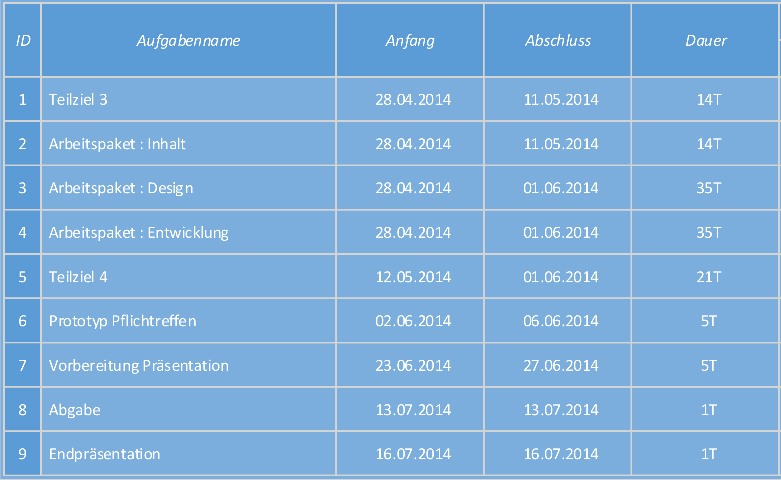
\includegraphics[width=\linewidth]{zeitplan_1}

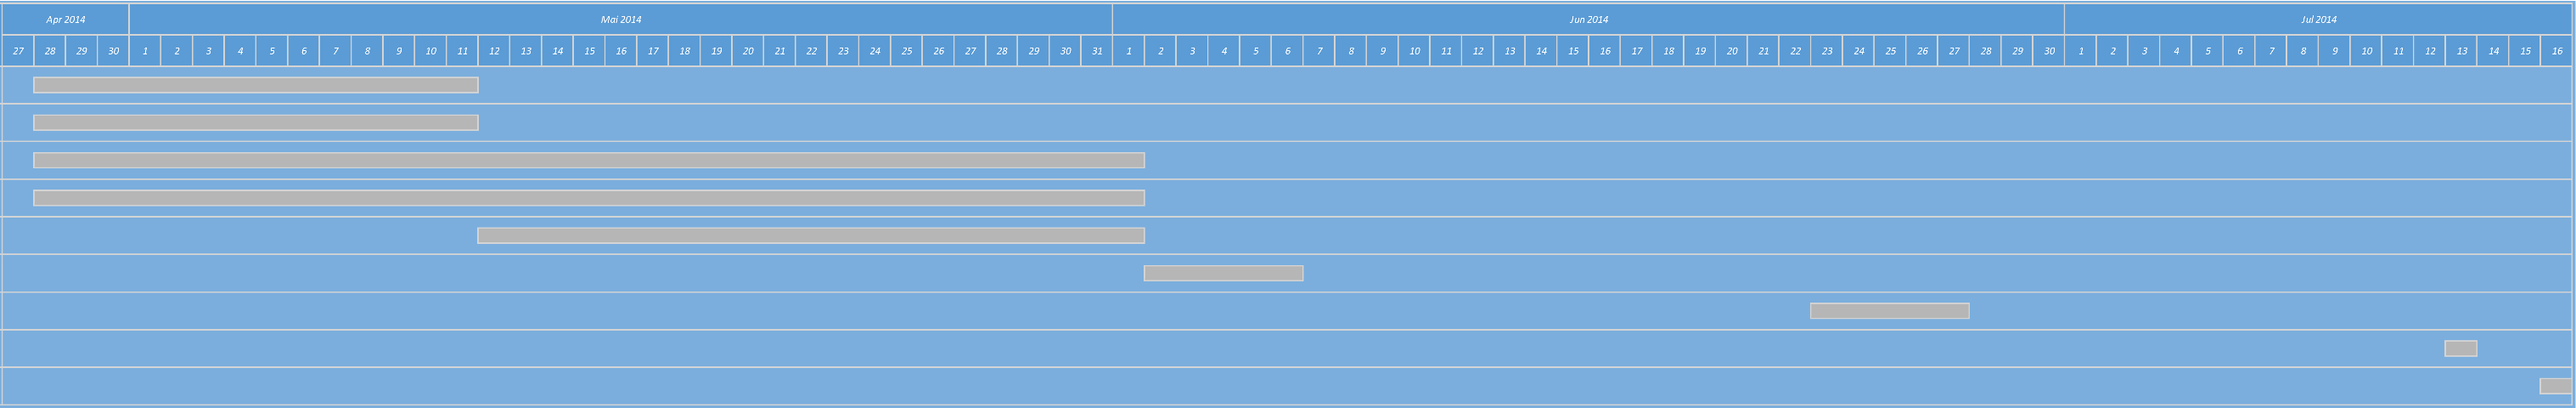
\includegraphics[width=\linewidth]{zeitplan_2}


\TOP{Inhalte - Aufbau}

Der Spieler durchläuft den ganzen Müllkreislauf, der mindestens vom Einkaufen über die Mülltrennung, Müllabfuhr, Müllverarbeitung sowie dem Recycling und dem Wiederverkauf besteht.
Über das Hauptmenü kann der Spieler seinen momentanen Fortschritt sehen bzw. sehen wo im Kreislauf er sich momentan befindet und ggf. zu bereits besuchten Orten zurückspringen.
An jeder der Stationen des Kreislaufs erwarten den Spieler verschiedene Aufgaben bzw. Minispiele sowie Informationen zu der speziellen Thematik..

\begin{center}
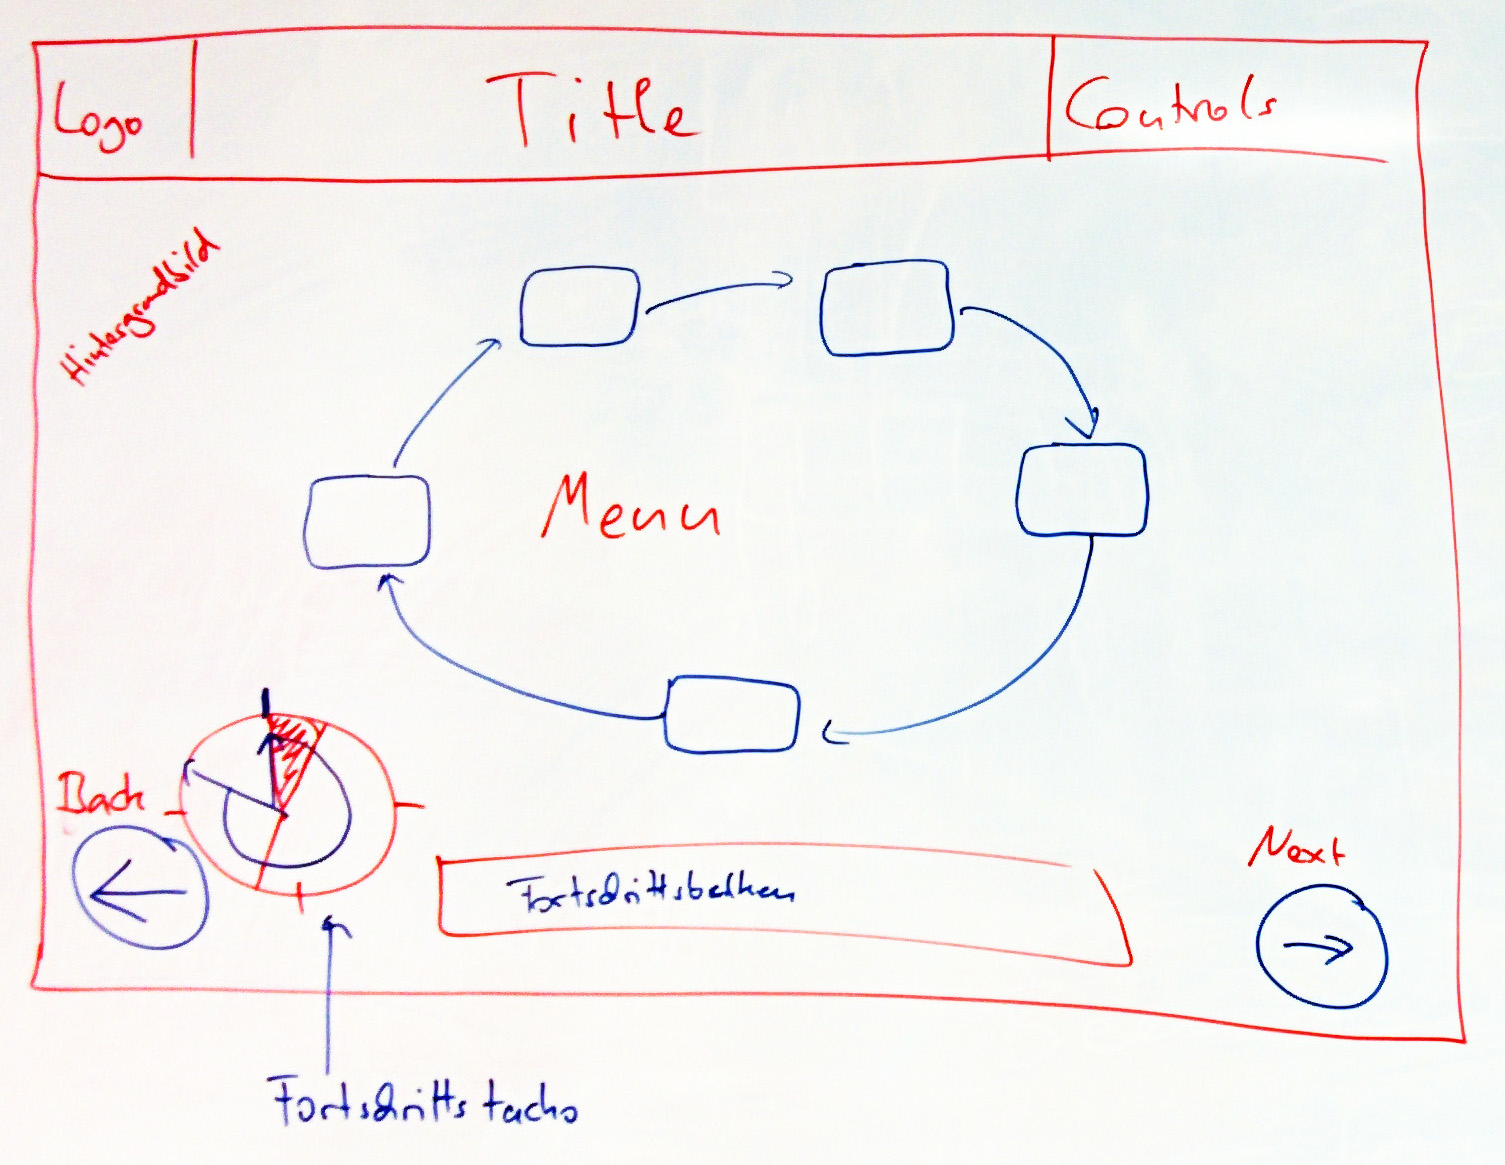
\includegraphics[width=.8\linewidth]{../mockups/menu}
\end{center}


\begin{center}
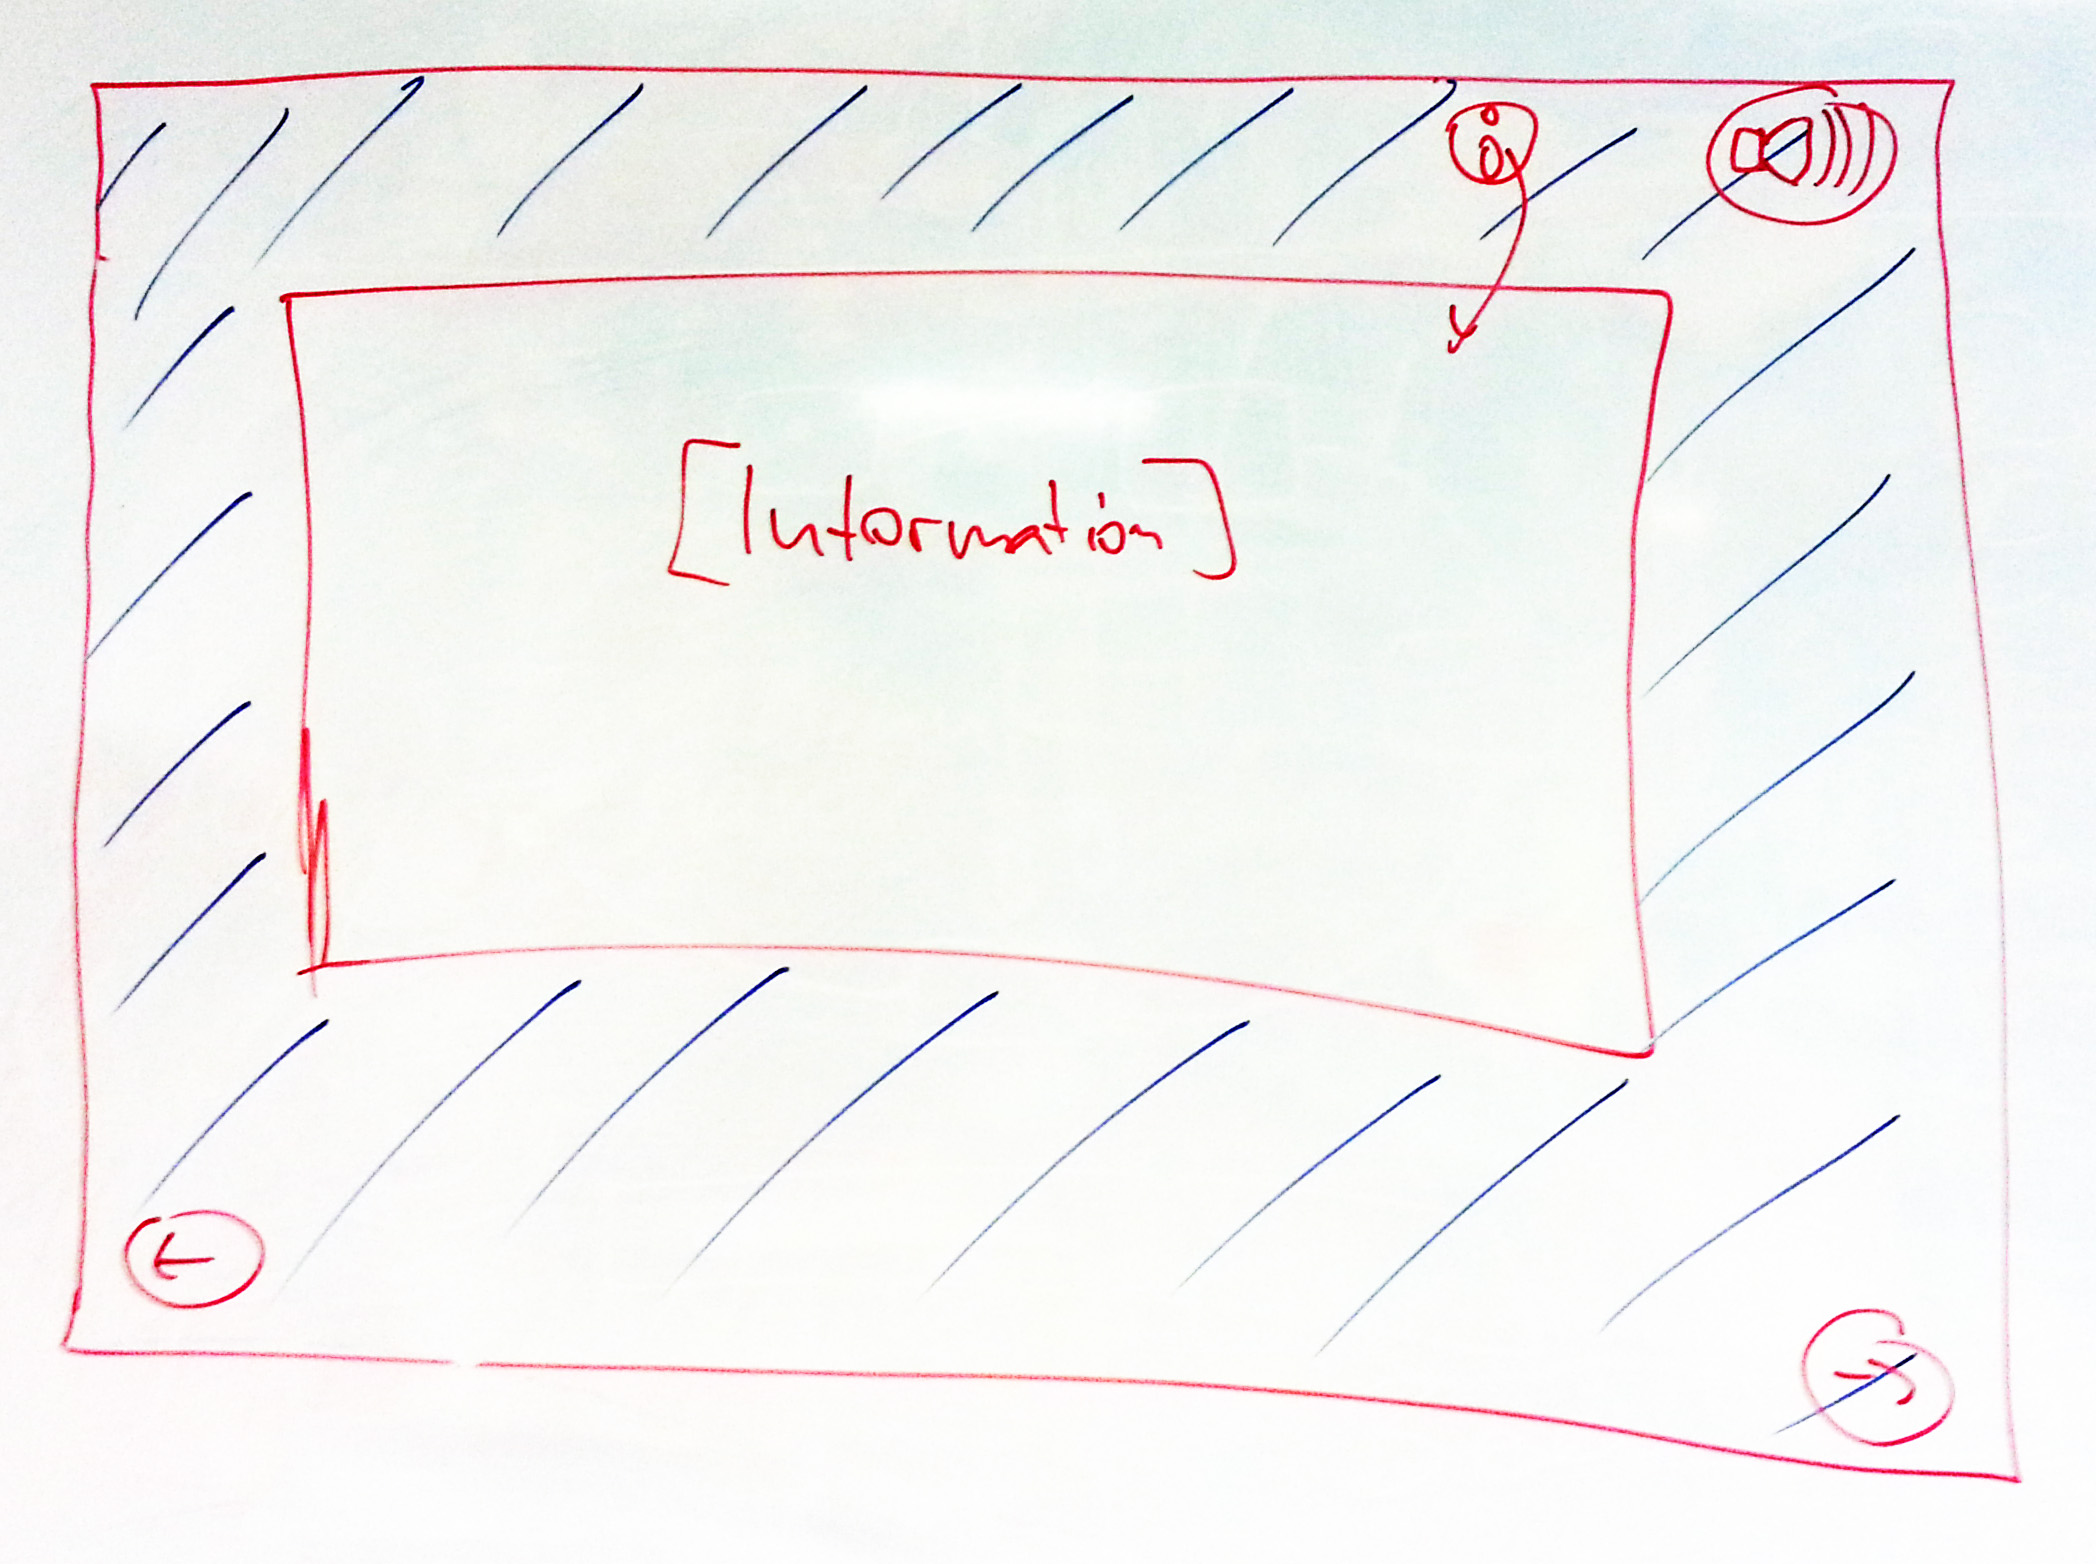
\includegraphics[width=.8\linewidth]{../mockups/lerninfo}
\end{center}

Erklärungen und Lerninhalten werden einheitlich nach der Wahl einer Station bildschirmfüllend dargestellt.
Der Spieler hat jedoch auch die Möglichkeit direkt zum Minispiel zu springen.

\begin{center}
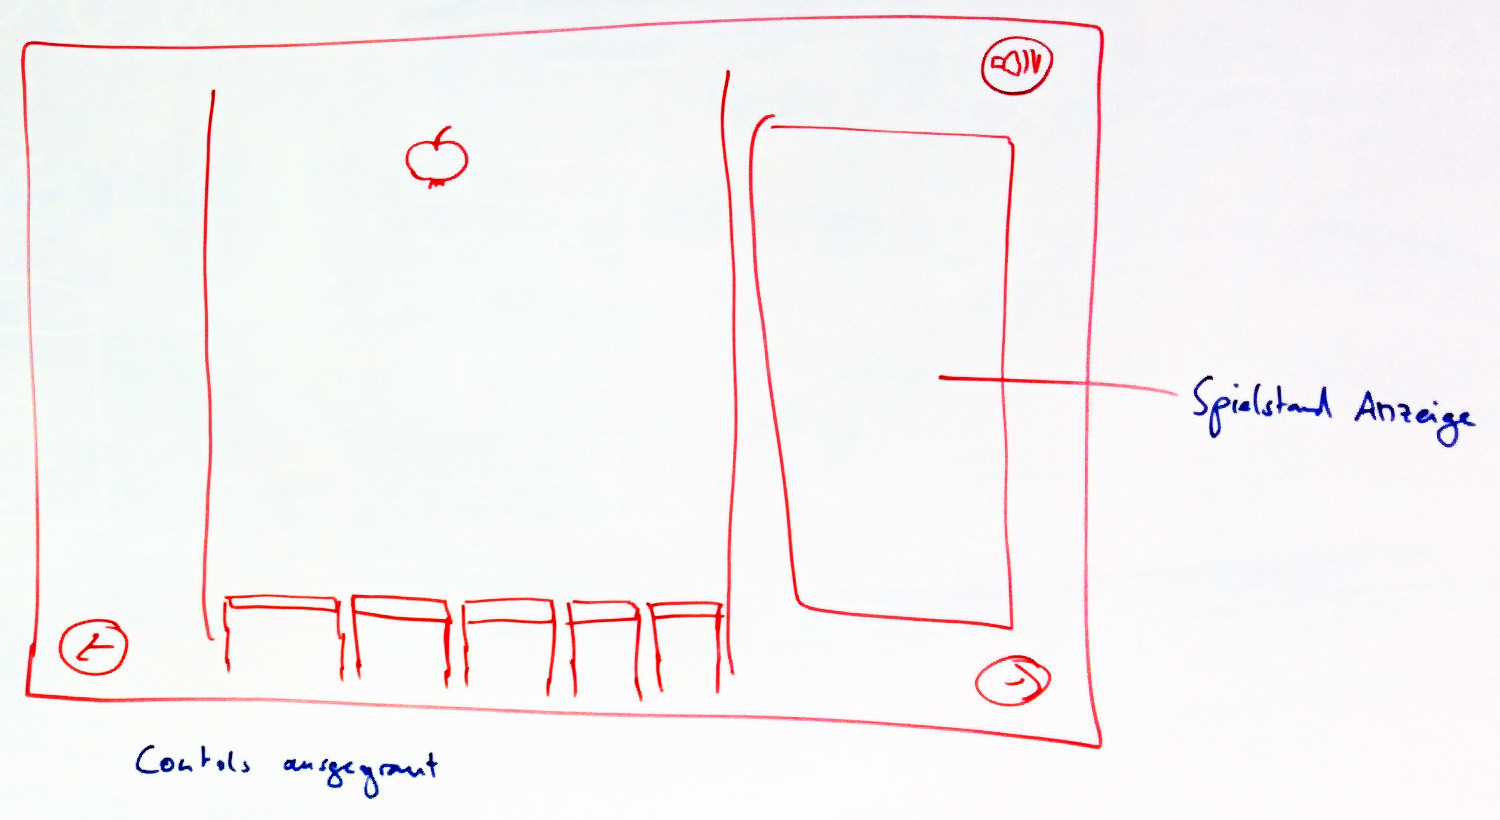
\includegraphics[width=.8\linewidth]{../mockups/minispiel}
\end{center}

Beispielhaft ist hier ein Auffangspiel dargestellt, in dem es darum geht, fallende Müllobjekte in die richtigen Mülleimer zu manövrieren.
Das Hauptinterface in Form des Menüs in der oberen rechten Ecke und am unteren Bildschirmrand bleibt jedoch auf jedem Bildschirm erhalten.

\begin{center}
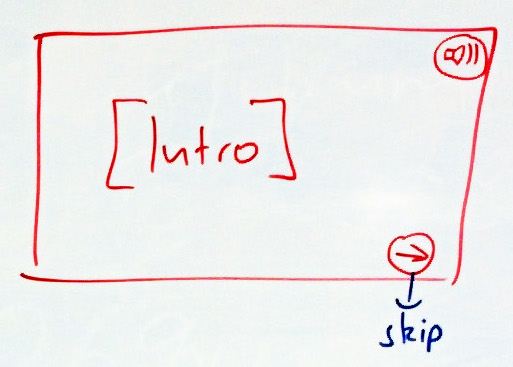
\includegraphics[width=.8\linewidth]{../mockups/intro}
\end{center}


\textbf{Die Stationen:}

\begin{enumerate}

	\item Einkaufen
	\begin{itemize}
		\item Verantwortungsvolles Einkaufen
		\begin{itemize}
			\item Sachen mit wenig Plastikverpackung
			\item Recyclebare Verpackung
			\item bevorzugt regionale Produkte
		\end{itemize}
		\item Minispiel
		\begin{itemize}
			\item Anhand von Fragen, der persönlichen Einschätzung nach, aus verschiedenen Regalen im Supermarkt Produkte wählen
			\item Analyse des Kaufverhaltens und Informationen zur Verbesserung
		\end{itemize}
	\end{itemize}

	\item Mülltrennung
	\begin{itemize}
		\item Verschiedene Müllsorten und ihre richtige Entsorgung
		\item Minispiel
		\begin{itemize}
			\item Müllsortieren
			\item Der Spieler bekommt verschiedenen Müll und sortiert diesen der richtigen Entsorgungstätte zu
			\item Steuerung an Tetris angelehnt
			\item Auswertung nach dem Spielende und Informationen zu dem falsch entsorgtem Müll
		\end{itemize}
	\end{itemize}

	\item Müllabfuhr
	\begin{itemize}
		\item Trennen zwischen Deponie, Verbrennungsanlage, Recycling, etc.
		\item Welche Organisationen holen den Müll ab/nehmen ihn an?
		\begin{itemize}
			\item Staatliche
			\item Private
		\end{itemize}
	\end{itemize}

	\item Müllverarbeitung
	\begin{itemize}
		\item Was passiert in der
		\begin{itemize}
			\item Mülldeponie
			\item Verbrennungsanlage
		\end{itemize}
		\item Wo wird nicht recyclebarer Müll verstaut?
		\item Was für Schaden wird durch Müll verursacht?
		\begin{itemize}
			\item Grundwasserverschmutzung
			\item Gefahren von Endlagern
			\item Problematik in 3. Welt Ländern
		\end{itemize}
	\end{itemize}

	\item Recycling
	\begin{itemize}
		\item Wie funktioniert das Recyclen verschiedenen Mülls?
		\item Wie viel des Grundmaterials kann am Ende wiederverwertet werden?
		\item Wofür kann man es noch verwenden?
		\item Minispiel
		\begin{itemize}
			\item Der Spieler muss aus recyclelten Rohstoffen bzw. Gegenständen neue Sachen herstellen
		\end{itemize}
	\end{itemize}


\end{enumerate}



\end{enumerate}


% das ist herrlich kompliziert, aber es klappt! das ist alles was zaehlt! :D
\definecolor{dgreen}{rgb}{0.549,0.776,0.247}
\makeatletter
\def\footrule{{
  \vskip-\footruleskip\vskip-\footrulewidth
  \color{\footrulecolor}
  \hrule\@width\headwidth\@height
  \footrulewidth\vskip\footruleskip
}}
\makeatother
\renewcommand{\footrulewidth}{3pt}
\newcommand{\footrulecolor}{dgreen}

\end{document}
